\usetikzlibrary{patterns}
\begin{figure}[ht]
    \centering
   

% Pattern Info
 
\tikzset{
pattern size/.store in=\mcSize, 
pattern size = 5pt,
pattern thickness/.store in=\mcThickness, 
pattern thickness = 0.3pt,
pattern radius/.store in=\mcRadius, 
pattern radius = 1pt}
\makeatletter
\pgfutil@ifundefined{pgf@pattern@name@_8sa0p8rq6}{
\pgfdeclarepatternformonly[\mcThickness,\mcSize]{_8sa0p8rq6}
{\pgfqpoint{0pt}{0pt}}
{\pgfpoint{\mcSize+\mcThickness}{\mcSize+\mcThickness}}
{\pgfpoint{\mcSize}{\mcSize}}
{
\pgfsetcolor{\tikz@pattern@color}
\pgfsetlinewidth{\mcThickness}
\pgfpathmoveto{\pgfqpoint{0pt}{0pt}}
\pgfpathlineto{\pgfpoint{\mcSize+\mcThickness}{\mcSize+\mcThickness}}
\pgfusepath{stroke}
}}
\makeatother

% Pattern Info
 
\tikzset{
pattern size/.store in=\mcSize, 
pattern size = 5pt,
pattern thickness/.store in=\mcThickness, 
pattern thickness = 0.3pt,
pattern radius/.store in=\mcRadius, 
pattern radius = 1pt}
\makeatletter
\pgfutil@ifundefined{pgf@pattern@name@_whu02zlbn}{
\pgfdeclarepatternformonly[\mcThickness,\mcSize]{_whu02zlbn}
{\pgfqpoint{0pt}{0pt}}
{\pgfpoint{\mcSize+\mcThickness}{\mcSize+\mcThickness}}
{\pgfpoint{\mcSize}{\mcSize}}
{
\pgfsetcolor{\tikz@pattern@color}
\pgfsetlinewidth{\mcThickness}
\pgfpathmoveto{\pgfqpoint{0pt}{0pt}}
\pgfpathlineto{\pgfpoint{\mcSize+\mcThickness}{\mcSize+\mcThickness}}
\pgfusepath{stroke}
}}
\makeatother
\tikzset{every picture/.style={line width=0.75pt}} %set default line width to 0.75pt        

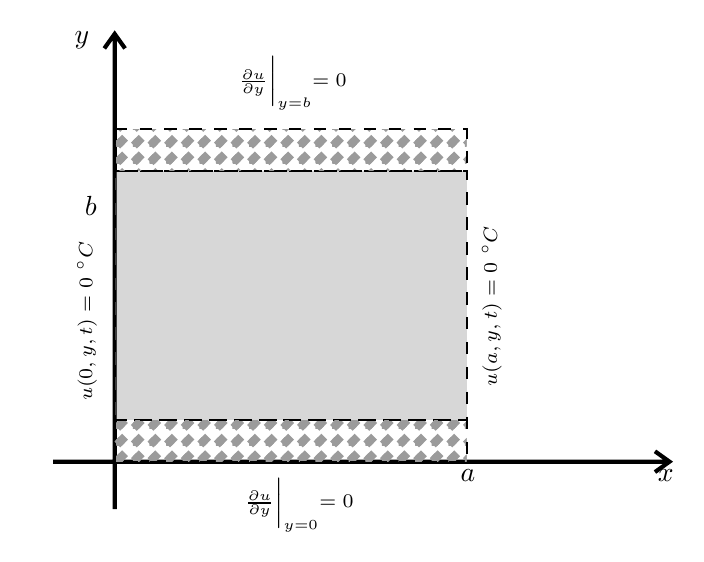
\begin{tikzpicture}[x=0.75pt,y=0.75pt,yscale=-1,xscale=1]
%uncomment if require: \path (0,300); %set diagram left start at 0, and has height of 300

%Shape: Axis 2D [id:dp8836634611392435] 
\draw [color={rgb, 255:red, 0; green, 0; blue, 0 }  ,draw opacity=1 ][line width=1.5]  (68.13,229.81) -- (365.13,229.81)(97.83,23.71) -- (97.83,252.71) (358.13,224.81) -- (365.13,229.81) -- (358.13,234.81) (92.83,30.71) -- (97.83,23.71) -- (102.83,30.71)  ;
%Shape: Rectangle [id:dp6128441923797413] 
\draw  [color={rgb, 255:red, 0; green, 0; blue, 0 }  ,draw opacity=1 ][fill={rgb, 255:red, 155; green, 155; blue, 155 }  ,fill opacity=0.4 ][dash pattern={on 4.5pt off 4.5pt}] (97.83,89.71) -- (267.43,89.71) -- (267.43,209.81) -- (97.83,209.81) -- cycle ;
%Shape: Rectangle [id:dp0645349541513307] 
\draw  [color={rgb, 255:red, 0; green, 0; blue, 0 }  ,draw opacity=1 ][pattern=_8sa0p8rq6,pattern size=6pt,pattern thickness=3pt,pattern radius=0pt, pattern color={rgb, 255:red, 155; green, 155; blue, 155}][dash pattern={on 4.5pt off 4.5pt}] (97.83,69.71) -- (267.43,69.71) -- (267.43,89.71) -- (97.83,89.71) -- cycle ;
%Shape: Rectangle [id:dp11129610169623028] 
\draw  [color={rgb, 255:red, 0; green, 0; blue, 0 }  ,draw opacity=1 ][pattern=_whu02zlbn,pattern size=6pt,pattern thickness=3pt,pattern radius=0pt, pattern color={rgb, 255:red, 155; green, 155; blue, 155}][dash pattern={on 4.5pt off 4.5pt}] (97.83,209.81) -- (267.43,209.81) -- (267.43,229.81) -- (97.83,229.81) -- cycle ;

% Text Node
\draw (56.41,118.69) node [anchor=north west][inner sep=0.75pt]  [color={rgb, 255:red, 255; green, 255; blue, 255 }  ,opacity=1 ] [align=left] {11};
% Text Node
\draw (358,232.21) node [anchor=north west][inner sep=0.75pt]    {$x$};
% Text Node
\draw (77,21.21) node [anchor=north west][inner sep=0.75pt]    {$y$};
% Text Node
\draw (78.19,202) node [anchor=north west][inner sep=0.75pt]  [font=\scriptsize,rotate=-270.03]  {$u( 0,y,t) =0\ ^{\circ } C$};
% Text Node
\draw (263,232.21) node [anchor=north west][inner sep=0.75pt]    {$a$};
% Text Node
\draw (82,100.21) node [anchor=north west][inner sep=0.75pt]    {$b$};
% Text Node
\draw (273.19,195) node [anchor=north west][inner sep=0.75pt]  [font=\scriptsize,rotate=-270.03]  {$u( a,y,t) =0\ ^{\circ } C$};
% Text Node
\draw (156,32.21) node [anchor=north west][inner sep=0.75pt]  [font=\scriptsize]  {$\frac{\partial u}{\partial y}\Bigl|_{y=b} =0$};
% Text Node
\draw (159,235.21) node [anchor=north west][inner sep=0.75pt]  [font=\scriptsize]  {$\frac{\partial u}{\partial y}\Bigl|_{y=0} =0$};


\end{tikzpicture}
   \caption{Placa rectangular metálica}
\end{figure}